\documentclass{standalone}
\usepackage{tikz}
\usetikzlibrary{patterns, positioning}


\begin{document}
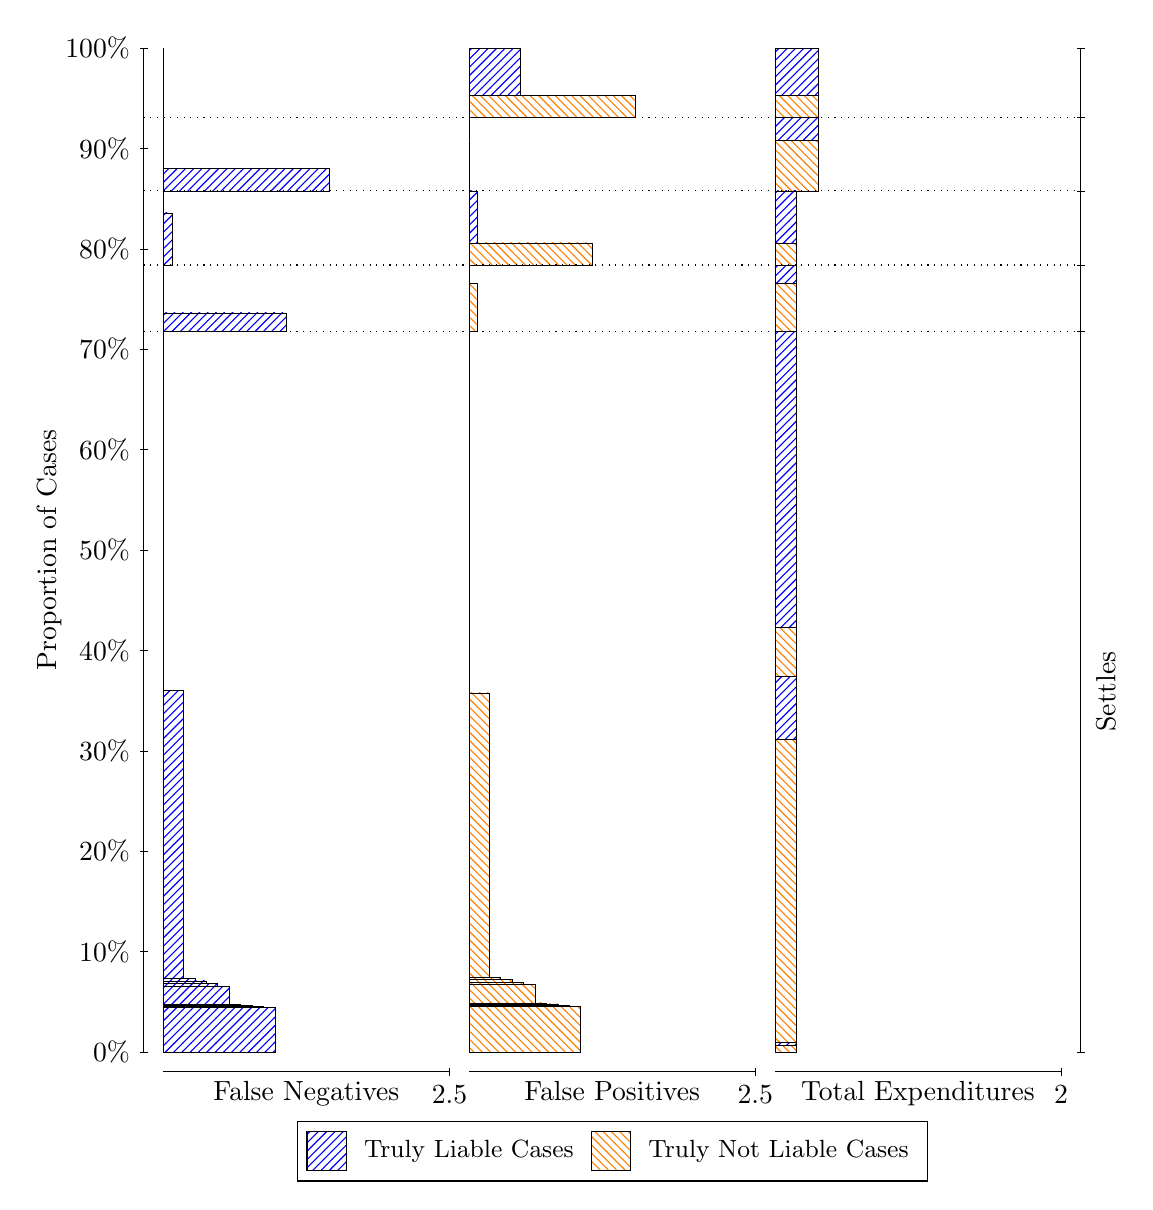
\begin{tikzpicture}
\draw[black, very thin] (1.5,1.75) -- (1.5,14.5);
\node[rotate=90, text=black, anchor=center] at (0.3, 8.125) {Proportion of Cases};
\draw[black, very thin] (1.45,1.75) -- (1.55,1.75);
\node[text=black, anchor=east] at (1.45, 1.75) {0\%};
\draw[black, very thin] (1.45,3.025) -- (1.55,3.025);
\node[text=black, anchor=east] at (1.45, 3.025) {10\%};
\draw[black, very thin] (1.45,4.3) -- (1.55,4.3);
\node[text=black, anchor=east] at (1.45, 4.3) {20\%};
\draw[black, very thin] (1.45,5.575) -- (1.55,5.575);
\node[text=black, anchor=east] at (1.45, 5.575) {30\%};
\draw[black, very thin] (1.45,6.85) -- (1.55,6.85);
\node[text=black, anchor=east] at (1.45, 6.85) {40\%};
\draw[black, very thin] (1.45,8.125) -- (1.55,8.125);
\node[text=black, anchor=east] at (1.45, 8.125) {50\%};
\draw[black, very thin] (1.45,9.4) -- (1.55,9.4);
\node[text=black, anchor=east] at (1.45, 9.4) {60\%};
\draw[black, very thin] (1.45,10.675) -- (1.55,10.675);
\node[text=black, anchor=east] at (1.45, 10.675) {70\%};
\draw[black, very thin] (1.45,11.95) -- (1.55,11.95);
\node[text=black, anchor=east] at (1.45, 11.95) {80\%};
\draw[black, very thin] (1.45,13.225) -- (1.55,13.225);
\node[text=black, anchor=east] at (1.45, 13.225) {90\%};
\draw[black, very thin] (1.45,14.5) -- (1.55,14.5);
\node[text=black, anchor=east] at (1.45, 14.5) {100\%};

\draw[black, very thin] (13.4,1.75) -- (13.4,14.5);
\draw[black, very thin] (13.35,1.75) -- (13.45,1.75);
\node[anchor=west] at (13.35, 1.75) {};
\draw[black, very thin] (13.35,10.904) -- (13.45,10.904);
\node[anchor=west] at (13.35, 10.904) {};
\draw[black, very thin] (13.35,11.744) -- (13.45,11.744);
\node[anchor=west] at (13.35, 11.744) {};
\draw[black, very thin] (13.35,12.687) -- (13.45,12.687);
\node[anchor=west] at (13.35, 12.687) {};
\draw[black, very thin] (13.35,13.615) -- (13.45,13.615);
\node[anchor=west] at (13.35, 13.615) {};
\draw[black, very thin] (13.35,14.5) -- (13.45,14.5);
\node[anchor=west] at (13.35, 14.5) {};

\draw[black, very thin, pattern color=blue, pattern=north east lines] (1.75,1.75) rectangle (3.167,2.3201);
\draw[black, very thin, pattern color=blue, pattern=north east lines] (1.75,2.3201) rectangle (3.0217,2.3308);
\draw[black, very thin, pattern color=blue, pattern=north east lines] (1.75,2.3308) rectangle (2.8763,2.3433);
\draw[black, very thin, pattern color=blue, pattern=north east lines] (1.75,2.3433) rectangle (2.731,2.3569);
\draw[black, very thin, pattern color=blue, pattern=north east lines] (1.75,2.3569) rectangle (2.5857,2.5858);
\draw[black, very thin, pattern color=blue, pattern=north east lines] (1.75,2.5858) rectangle (2.4403,2.6191);
\draw[black, very thin, pattern color=blue, pattern=north east lines] (1.75,2.6191) rectangle (2.295,2.6528);
\draw[black, very thin, pattern color=blue, pattern=north east lines] (1.75,2.6528) rectangle (2.1497,2.6858);
\draw[black, very thin, pattern color=blue, pattern=north east lines] (1.75,2.6858) rectangle (2.0043,6.3437);
\draw[black, very thin, pattern color=orange, pattern=north west lines] (1.75,6.3437) rectangle (1.75,10.904);
\draw[black, very thin, pattern color=blue, pattern=north east lines] (1.75,10.904) rectangle (3.3123,11.137);
\draw[black, very thin, pattern color=orange, pattern=north west lines] (1.75,11.137) rectangle (1.75,11.744);
\draw[black, very thin, pattern color=blue, pattern=north east lines] (1.75,11.744) rectangle (1.859,12.406);
\draw[black, very thin, pattern color=orange, pattern=north west lines] (1.75,12.406) rectangle (1.75,12.687);
\draw[black, very thin, pattern color=blue, pattern=north east lines] (1.75,12.687) rectangle (3.8573,12.973);
\draw[black, very thin, pattern color=orange, pattern=north west lines] (1.75,12.973) rectangle (1.75,13.615);
\draw[black, very thin, pattern color=orange, pattern=north west lines] (1.75,13.615) rectangle (1.75,13.901);
\draw[black, very thin, pattern color=blue, pattern=north east lines] (1.75,13.901) rectangle (1.75,14.5);
\draw[black, very thin, pattern color=orange, pattern=north west lines] (5.6333,1.75) rectangle (7.0503,2.3311);
\draw[black, very thin, pattern color=orange, pattern=north west lines] (5.6333,2.3311) rectangle (6.905,2.345);
\draw[black, very thin, pattern color=orange, pattern=north west lines] (5.6333,2.345) rectangle (6.7597,2.3597);
\draw[black, very thin, pattern color=orange, pattern=north west lines] (5.6333,2.3597) rectangle (6.6143,2.3742);
\draw[black, very thin, pattern color=orange, pattern=north west lines] (5.6333,2.3742) rectangle (6.469,2.6055);
\draw[black, very thin, pattern color=orange, pattern=north west lines] (5.6333,2.6055) rectangle (6.3237,2.6065);
\draw[black, very thin, pattern color=orange, pattern=north west lines] (5.6333,2.6065) rectangle (6.3237,2.6377);
\draw[black, very thin, pattern color=orange, pattern=north west lines] (5.6333,2.6377) rectangle (6.1783,2.6671);
\draw[black, very thin, pattern color=orange, pattern=north west lines] (5.6333,2.6671) rectangle (6.033,2.6932);
\draw[black, very thin, pattern color=orange, pattern=north west lines] (5.6333,2.6932) rectangle (5.8877,6.3098);
\draw[black, very thin, pattern color=blue, pattern=north east lines] (5.6333,6.3098) rectangle (5.6333,10.904);
\draw[black, very thin, pattern color=orange, pattern=north west lines] (5.6333,10.904) rectangle (5.7423,11.51);
\draw[black, very thin, pattern color=blue, pattern=north east lines] (5.6333,11.51) rectangle (5.6333,11.744);
\draw[black, very thin, pattern color=orange, pattern=north west lines] (5.6333,11.744) rectangle (7.1957,12.025);
\draw[black, very thin, pattern color=blue, pattern=north east lines] (5.6333,12.025) rectangle (5.7423,12.687);
\draw[black, very thin, pattern color=orange, pattern=north west lines] (5.6333,12.687) rectangle (5.6333,13.328);
\draw[black, very thin, pattern color=blue, pattern=north east lines] (5.6333,13.328) rectangle (5.6333,13.615);
\draw[black, very thin, pattern color=orange, pattern=north west lines] (5.6333,13.615) rectangle (7.7407,13.901);
\draw[black, very thin, pattern color=blue, pattern=north east lines] (5.6333,13.901) rectangle (6.2873,14.5);
\draw[black, very thin, pattern color=orange, pattern=north west lines] (9.5167,1.75) rectangle (9.7892,1.8377);
\draw[black, very thin, pattern color=blue, pattern=north east lines] (9.5167,1.8377) rectangle (9.7892,1.8745);
\draw[black, very thin, pattern color=orange, pattern=north west lines] (9.5167,1.8745) rectangle (9.7892,5.7225);
\draw[black, very thin, pattern color=blue, pattern=north east lines] (9.5167,5.7225) rectangle (9.7892,6.5215);
\draw[black, very thin, pattern color=orange, pattern=north west lines] (9.5167,6.5215) rectangle (9.7892,7.1456);
\draw[black, very thin, pattern color=blue, pattern=north east lines] (9.5167,7.1456) rectangle (9.7892,10.904);
\draw[black, very thin, pattern color=orange, pattern=north west lines] (9.5167,10.904) rectangle (9.7892,11.51);
\draw[black, very thin, pattern color=blue, pattern=north east lines] (9.5167,11.51) rectangle (9.7892,11.744);
\draw[black, very thin, pattern color=orange, pattern=north west lines] (9.5167,11.744) rectangle (9.7892,12.025);
\draw[black, very thin, pattern color=blue, pattern=north east lines] (9.5167,12.025) rectangle (9.7892,12.687);
\draw[black, very thin, pattern color=orange, pattern=north west lines] (9.5167,12.687) rectangle (10.062,13.328);
\draw[black, very thin, pattern color=blue, pattern=north east lines] (9.5167,13.328) rectangle (10.062,13.615);
\draw[black, very thin, pattern color=orange, pattern=north west lines] (9.5167,13.615) rectangle (10.062,13.901);
\draw[black, very thin, pattern color=blue, pattern=north east lines] (9.5167,13.901) rectangle (10.062,14.5);
\draw[black, dotted] (1.5,10.904) -- (13.4,10.904);
\draw[black, dotted] (1.5,11.744) -- (13.4,11.744);
\draw[black, dotted] (1.5,12.687) -- (13.4,12.687);
\draw[black, dotted] (1.5,13.615) -- (13.4,13.615);
\draw[black, very thin] (1.75,1.5) -- (5.3833,1.5);
\node[text=black, anchor=north] at (3.5667, 1.5) {False Negatives};
\draw[black, very thin] (5.3833,1.45) -- (5.3833,1.55);
\node[text=black, anchor=north] at (5.3833, 1.45) {2.5};

\draw[black, very thin] (5.6333,1.5) -- (9.2667,1.5);
\node[text=black, anchor=north] at (7.45, 1.5) {False Positives};
\draw[black, very thin] (9.2667,1.45) -- (9.2667,1.55);
\node[text=black, anchor=north] at (9.2667, 1.45) {2.5};

\draw[black, very thin] (9.5167,1.5) -- (13.15,1.5);
\node[text=black, anchor=north] at (11.333, 1.5) {Total Expenditures};
\draw[black, very thin] (13.15,1.45) -- (13.15,1.55);
\node[text=black, anchor=north] at (13.15, 1.45) {2};

\node[text=black, centered, rotate=90] at (13.72, 6.3268) {Settles};





\draw (7.449999999999999,1.5) node[draw=none] (baseCoordinate) {};
\begin{scope}[align=center]
        \matrix[scale=0.5, draw=black, below=0.5cm of baseCoordinate, nodes={draw}, column sep=0.1cm]{
            \node[rectangle, draw, minimum width=0.5cm, minimum height=0.5cm, pattern color=blue, pattern=north east lines] {}; &
            \node[draw=none, font=\small, text=black] (B) {Truly Liable Cases}; &
            \node[rectangle, draw, minimum width=0.5cm, minimum height=0.5cm, pattern color=orange, pattern=north west lines] {}; &
            \node[draw=none, font=\small, text=black] (B) {Truly Not Liable Cases}; \\
            };
\end{scope}

\end{tikzpicture}
\end{document}